\section{Results and Analysis}
This section presents the results of the experiments conducted in this study, organized into subsections focusing on specific aspects of the project. Initially, the performance of Decision Tree models is compared across the DAIC-WOZ and EATD datasets. In the subsequent TCC section, only the DAIC-WOZ dataset is used for evaluation.

\subsection{Model Performance - DT}
This subsection evaluates the performance of DT models across two datasets: DAIC-WOZ and EATD. While the models showcased excellent performance on the DAIC-WOZ dataset with an accuracy of 98.11\%, precision of 97.00\%, recall of 100.00\%, and F1-score of 98.46\% on the training set (Tables \ref{table:classification_report_train_daic} and Figures \ref{fig:confusion_matrices_daic}, \ref{table:classification_report_dev_daic}), a significant drop in performance was observed on the development set.

Particularly, the development set for the DAIC-WOZ dataset displayed only a 66\% accuracy (Table \ref{table:classification_report_dev_daic}), suggesting issues with the model's ability to generalize to new data. 

Similarly, for the EATD dataset, while the training results were promising with an accuracy of 87\% (Table \ref{table:classification_report_train_eatd}), the development set results were considerably lower, achieving only a 68\% accuracy (Table \ref{table:classification_report_dev_eatd}). This performance decrement underscores the necessity to consider alternative modeling strategies that might improve generalization across unseen datasets.


\begin{table}[H]
    \centering
    \scalebox{0.8}{% Scale the table to 50% of the original size
    \begin{tabular}{|c|c|c|c|c|}
    \hline
    \textbf{Class} & \textbf{Precision} & \textbf{Recall} & \textbf{F1-score} & \textbf{Support} \\ \hline
    0              & 0.97               & 1.00            & 0.99              & 76               \\ \hline
    1              & 1.00               & 0.93            & 0.97              & 30               \\ \hline
    \multicolumn{5}{|c|}{\textbf{Accuracy}: 0.98 \textbf{of} 106}                         \\ \hline
    \multicolumn{5}{|c|}{\textbf{Macro Avg}: Precision 0.99, Recall 0.97, F1-score 0.98} \\ \hline
    \multicolumn{5}{|c|}{\textbf{Weighted Avg}: Precision 0.98, Recall 0.98, F1-score 0.98} \\ \hline
    \end{tabular}}
    \caption{Classification Report on Training Set - DAIC}
    \label{table:classification_report_train_daic}
\end{table}


\begin{table}[H]
    \centering
    \scalebox{0.8}{% Scale the table to 50% of the original size
    \begin{tabular}{|c|c|c|c|c|}
    \hline
    \textbf{Class} & \textbf{Precision} & \textbf{Recall} & \textbf{F1-score} & \textbf{Support} \\ \hline
    0              & 0.76               & 0.65            & 0.70              & 20               \\ \hline
    1              & 0.53               & 0.67            & 0.59              & 12               \\ \hline
    \multicolumn{5}{|c|}{\textbf{Accuracy}: 0.66 \textbf{of} 32}                          \\ \hline
    \multicolumn{5}{|c|}{\textbf{Macro Avg}: Precision 0.65, Recall 0.66, F1-score 0.65} \\ \hline
    \multicolumn{5}{|c|}{\textbf{Weighted Avg}: Precision 0.68, Recall 0.66, F1-score 0.66} \\ \hline
    \end{tabular}}
    \caption{Classification Report on Development Set - DAIC}
    \label{table:classification_report_dev_daic}
\end{table}

\begin{figure}[H]
    \centering
    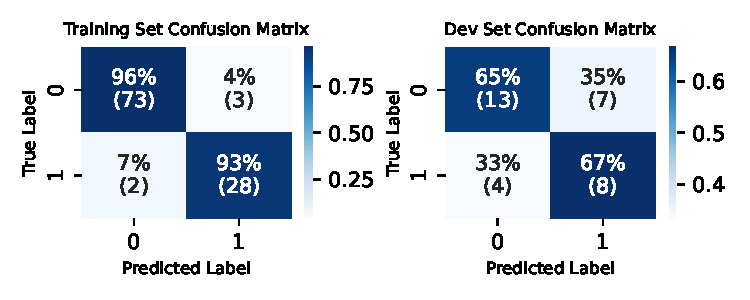
\includegraphics[width=0.45\textwidth]{vis_pdf/daic_all_confusion_matrices.pdf} % Adjust the scale to fit the page
    \caption{Confusion Matrices for Development Set (DAIC-WOZ)}
    \label{fig:confusion_matrices_daic}
\end{figure}


%EATD

%TRAIN

\begin{table}[H]
    \centering
    \scalebox{0.8}{% Scale the table to 80% of the original size
    \begin{tabular}{|c|c|c|c|c|}
    \hline
    \textbf{Class} & \textbf{Precision} & \textbf{Recall} & \textbf{F1-score} & \textbf{Support} \\ \hline
    0              & 0.96               & 0.84            & 0.90              & 56               \\ \hline
    1              & 0.74               & 0.93            & 0.82              & 27               \\ \hline
    \multicolumn{5}{|c|}{\textbf{Accuracy}: 0.87 \textbf{of} 83}                        \\ \hline
    \multicolumn{5}{|c|}{\textbf{Macro Avg}: Precision 0.85, Recall 0.88, F1-score 0.86} \\ \hline
    \multicolumn{5}{|c|}{\textbf{Weighted Avg}: Precision 0.89, Recall 0.87, F1-score 0.87} \\ \hline
    \end{tabular}}
    \caption{Classification Report on Training Set - EATD}
    \label{table:classification_report_train_eatd}
\end{table}



\begin{table}[H]
    \centering
    \scalebox{0.8}{% Scale the table to 80% of the original size
    \begin{tabular}{|c|c|c|c|c|}
    \hline
    \textbf{Class} & \textbf{Precision} & \textbf{Recall} & \textbf{F1-score} & \textbf{Support} \\ \hline
    0              & 0.71               & 0.88            & 0.79              & 52               \\ \hline
    1              & 0.54               & 0.27            & 0.36              & 26               \\ \hline
    \multicolumn{5}{|c|}{\textbf{Accuracy}: 0.68 \textbf{of} 78}                        \\ \hline
    \multicolumn{5}{|c|}{\textbf{Macro Avg}: Precision 0.62, Recall 0.58, F1-score 0.57} \\ \hline
    \multicolumn{5}{|c|}{\textbf{Weighted Avg}: Precision 0.65, Recall 0.68, F1-score 0.64} \\ \hline
    \end{tabular}}
    \caption{Classification Report on Development Set - EATD}
    \label{table:classification_report_dev_eatd}
\end{table}


\begin{figure}[H]
\centering
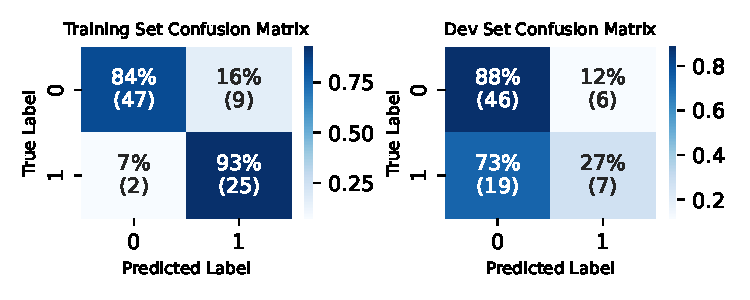
\includegraphics[width=0.45\textwidth]{vis_pdf/eatd_all_confusion_matrices.pdf} % Adjust the scale to fit the page
\caption{Confusion Matrices for Development Set (EATD)}
\label{fig:confusion_matrices_eatd}
\end{figure}

Worst to mention that when a DT was trained in both datasets the ANPVA choosed different features. 

\subsection{Model Performance - CNN}

In my experiments with various CNN models described in the literature, the models consistently underperformed, achieving only 50\% accuracy on the development set. A deeper investigation into the literature revealed that the models achieving high accuracy were trained and tested on data from the same participants, merely split into different sets. This means that the same participant's audio files were divided between the train and test sets. The visualization of this data splitting method is shown in Figure \ref{fig:train_test_split_problems}.

\begin{figure}[H]
    \centering
    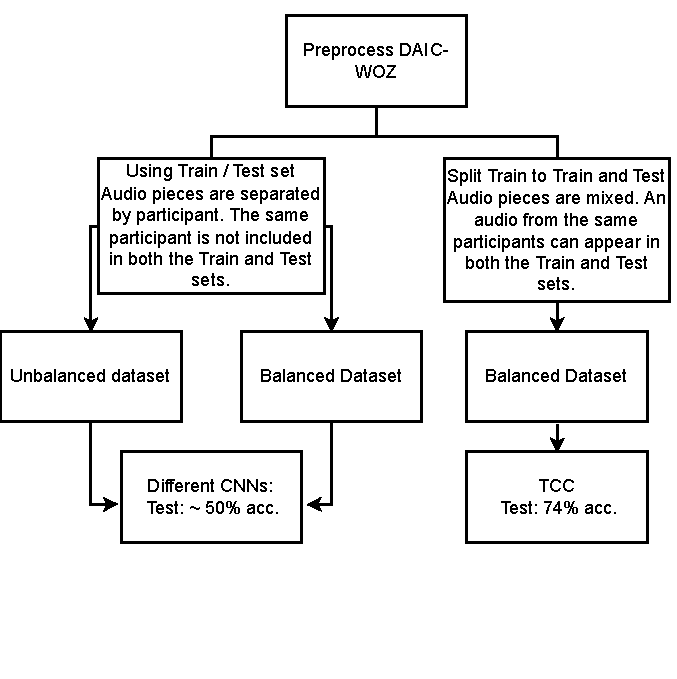
\includegraphics[width=0.45\textwidth]{vis_pdf/Train Test problem.drawio.pdf}
    \caption{Train/Test split strategies and their results (DAIC)}
    \label{fig:train_test_split_problems}
\end{figure}

The CNN models struggled to generalize when tasked with predicting new, unseen participants. The variance in accuracy across different CNN architectures is not discussed in this report. Instead, we focus on the results from the TCC model, detailed in Figure \ref{fig:confusion_matrices_TCC_daic}.
The training and validation accuracy and loss are depicted in Figure \ref{fig:training_TCC_daic}. The model underwent training for approximately 100 epochs, not to achieve the best possible accuracy but to demonstrate the model’s learning capability.
The model reached a 74\% accuracy on the development set, using a lightweight version of the architecture proposed by Yin et al.\cite{yin2023depression}. The evaluation metrics presented are based on the model's performance at its peak accuracy.

\begin{figure}[H]
    \centering
    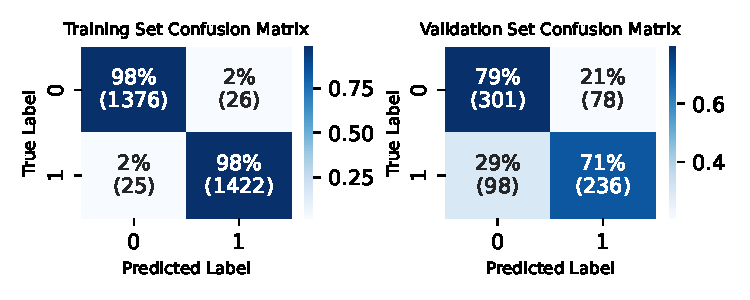
\includegraphics[width=0.45\textwidth]{vis_pdf/TCC_FINAL.pdf} % Adjust the scale to fit the page
    \caption{Confusion Matrices for Development Set (DAIC)}
    \label{fig:confusion_matrices_TCC_daic}
\end{figure}

\begin{figure}[H]
    \centering
    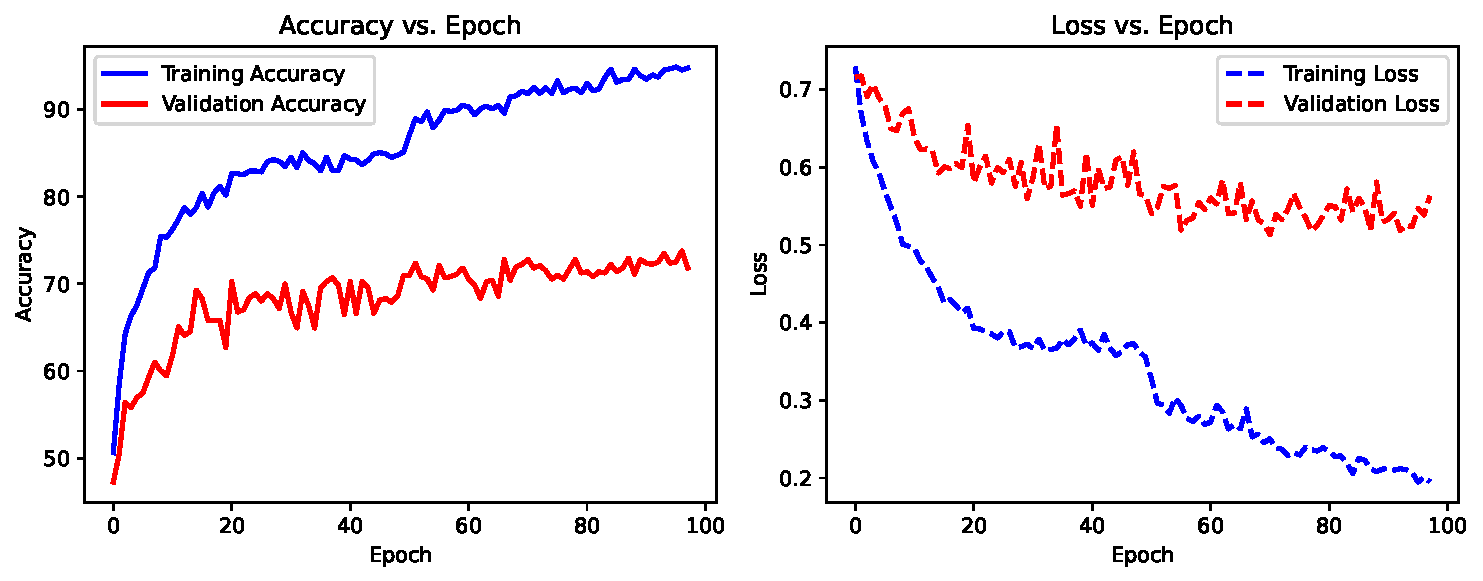
\includegraphics[width=0.45\textwidth]{vis_pdf/TCC_model_perf.pdf}
    \caption{TCC Training (DAIC)}
    \label{fig:training_TCC_daic}
\end{figure}



